\documentclass{article}

\usepackage{amsmath}
\usepackage{amsthm}
\usepackage{amsfonts}
\usepackage{thmtools}
\usepackage{stmaryrd}
\usepackage{natbib}
\usepackage{url}

\usepackage{tikz}


\declaretheorem[numbered=yes,name=Lemma]{lemma}
\declaretheorem[numbered=yes,name=Definition]{definition}

\newcommand{\update}[2]{[#1 \mapsto #2]}
\newcommand{\sem}[1]{\left\llbracket #1 \right\rrbracket}

%Math notation
\newcommand{\parfun}{\rightharpoonup}
\newcommand{\monfun}{\stackrel{\textit{\tiny{mon}}}{\longrightarrow}}
\newcommand{\defeq}{\stackrel{\textit{\tiny{def}}}{=}}
\newcommand{\union}{\mathbin{\cup}}
\DeclareMathOperator{\dom}{dom}

\newcommand{\undefined}{\mathit{undefined}}

\newcommand{\false}{\mathit{false}}
\newcommand{\true}{\mathit{true}}

%Variables
\newcommand{\var}[1]{\mathit{#1}}
\newcommand{\hv}{\var{hv}}
\newcommand{\rv}{\var{rv}}
\newcommand{\lv}{\var{lv}}
\newcommand{\pc}{\mathit{pc}}
\newcommand{\pcreg}{\mathrm{pc}}
\newcommand{\addr}{\var{a}}
\newcommand{\offset}{\var{offset}}
\newcommand{\word}{\var{w}}
\newcommand{\start}{\var{base}}
\newcommand{\addrend}{\var{end}}
\newcommand{\mem}{\var{mem}}
\newcommand{\reg}{\var{reg}}
\newcommand{\heapseg}{\var{hs}}
\newcommand{\heap}{\var{heap}}
\newcommand{\mode}{\var{mode}}
\newcommand{\perm}{\var{perm}}

\newcommand{\stdcap}[1][\perm]{\left(#1,\start,\addrend,\addr \right)}

%Memory projections
\newcommand{\plainproj}[1]{\mathrm{#1}}
\newcommand{\memheap}[1][\Phi]{#1.\plainproj{heap}}
\newcommand{\memreg}[1][\Phi]{#1.\plainproj{reg}}

\newcommand{\updateHeap}[3][\Phi]{#1\update{\plainproj{heap}.#2}{#3}}
\newcommand{\updateReg}[3][\Phi]{#1\update{\plainproj{reg}.#2}{#3}}

%Configuration end states
\newcommand{\failed}{\textsl{failed}}
\newcommand{\halted}{\textsl{halted}}

%Functions
\newcommand{\plainfun}[1]{\mathit{#1}}
\newcommand{\decode}{\plainfun{decode}}
\newcommand{\encode}{\plainfun{encode}}
\newcommand{\encodePerm}{\plainfun{encodePerm}}
\newcommand{\updatePcPerm}[1]{\plainfun{updatePcPerm}(#1)}
\newcommand{\executeAllowed}[1]{\plainfun{executeAllowed}(#1)}
\newcommand{\nonZero}[1]{\plainfun{nonZero}(#1)}
\newcommand{\readAllowed}[1]{\plainfun{readAllowed}(#1)}
\newcommand{\writeAllowed}[1]{\plainfun{writeAllowed}(#1)}
\newcommand{\withinBounds}[1]{\plainfun{withinBounds}(#1)}
\newcommand{\stdUpdatePc}[1]{\plainfun{updatePc(#1)}}

%World operations
\newcommand{\future}{\mathbin{\sqsupseteq}}
\newcommand{\heapSat}[3][\heap]{#1 :_{#2} #3}

%Assembly labels
\newcommand{\codelabel}[1]{\mathit{#1}}
\newcommand{\init}{\codelabel{init}}
\newcommand{\malloc}{\codelabel{malloc}}

%Type(s)
\newcommand{\type}[1]{\mathrm{#1}}
\newcommand{\asmType}{\plaindom{AsmType}}


%Domains
\newcommand{\plaindom}[1]{\mathrm{#1}}
\newcommand{\Caps}{\plaindom{Cap}}
\newcommand{\Words}{\plaindom{Word}}
\newcommand{\Addrs}{\plaindom{Addr}}
\newcommand{\Mems}{\plaindom{Mem}}
\newcommand{\RegName}{\plaindom{RegisterName}}
\newcommand{\Regs}{\plaindom{Reg}}
\newcommand{\Heaps}{\plaindom{Heap}}
\newcommand{\Confs}{\plaindom{Conf}}
\newcommand{\Instrs}{\plaindom{Instructions}}
\newcommand{\nats}{\mathbb{N}}
\newcommand{\ints}{\mathbb{Z}}
\newcommand{\Perms}{\plaindom{Perm}}

\newcommand{\RegionName}{\plaindom{RegionName}}
\newcommand{\Worlds}{\plaindom{World}}
\newcommand{\UPred}[1]{\plaindom{UPred}(#1)}

%LR
\newcommand{\intr}[2]{\mathcal{#1}\sem{#2}}
\newcommand{\valueintr}[1]{\intr{V}{#1}}
\newcommand{\exprintr}[1]{\intr{E}{#1}}
\newcommand{\contintr}[1]{\intr{K}{#1}}
\newcommand{\stdvr}{\valueintr{\asmType}}
\newcommand{\stder}{\exprintr{\asmType}}
\newcommand{\stdkr}{\contintr{\asmType}}
\newcommand{\observations}{\mathcal{O}}
\newcommand{\npair}[2][n]{\left(#1,#2 \right)}

%Reference register/heap
\newcommand{\refreg}[1]{\lfloor #1 \rfloor}
\newcommand{\refheap}[1]{\langle #1 \rangle_h}

%Instructions
%No arguments
\newcommand{\fail}{\instr{fail}}
\newcommand{\halt}{\instr{halt}}
%One argument
\newcommand{\instr}[1]{\mathtt{#1}}
\newcommand{\oneinstr}[2]{\instr{#1} \; #2}
\newcommand{\jmp}[1]{\oneinstr{jmp}{#1}}
%Two arguments
\newcommand{\twoinstr}[3]{\instr{#1} \; #2 \; #3}
\newcommand{\jnz}[2]{\twoinstr{jnz}{#1}{#2}}
\newcommand{\isptr}[2]{\twoinstr{isptr}{#1}{#2}}
\newcommand{\setptr}[2]{\twoinstr{setptr}{#1}{#2}}
\newcommand{\move}[2]{\twoinstr{move}{#1}{#2}}
\newcommand{\store}[2]{\twoinstr{store}{#1}{#2}}
\newcommand{\load}[2]{\twoinstr{load}{#1}{#2}}
\newcommand{\lea}[2]{\twoinstr{lea}{#1}{#2}}
%Three arguments
\newcommand{\threeinstr}[4]{\instr{#1} \; #2 \; #3 \; #4}
\newcommand{\restrict}[3]{\threeinstr{restrict}{#1}{#2}{#3}}
\newcommand{\subseg}[3]{\threeinstr{subseg}{#1}{#2}{#3}}
\newcommand{\plus}[3]{\threeinstr{plus}{#1}{#2}{#3}}

%Permissions
\newcommand{\plainperm}[1]{\mathrm{#1}}
\newcommand{\noperm}{\plainperm{o}}
\newcommand{\readonly}{\plainperm{ro}}
\newcommand{\readwrite}{\plainperm{rw}}
\newcommand{\exec}{\plainperm{rx}}
\newcommand{\entry}{\plainperm{e}}
\newcommand{\rwx}{\plainperm{rwx}}

%OP sem
\newcommand{\diverge}[1][n]{\not\Downarrow_{#1}}

\begin{document}
$\RegName$ contains $\pcreg$, but is otherwise some undefined, finite set.
\begin{align*}
\Addrs &::= \nats & & &
\Words &::= \Caps + \ints \\
\Regs  &::= \RegName \rightarrow \Words & & &
\Heaps &::= \Addrs \rightarrow \Words \\
\Perms &::= \{ \noperm, \readonly, \readwrite, \exec, \entry, \rwx\} & & &
\Mems  &::= \Regs \times \Heaps \\
\Caps  &::= \Perms \times \Addrs \times \Addrs \times \Addrs & & &
\Confs &::= \Mems + \{\failed, \halted \times \Mems\}
\end{align*}

\begin{figure}[!h]
  \centering
  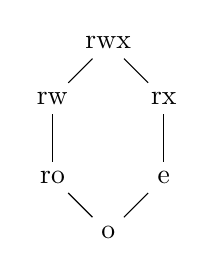
\begin{tikzpicture}[main node/.style={}]
  \node[main node] (1) {$\rwx$};
  \node[main node] (2) [below right of=1] {$\exec$};
  \node[main node] (3) [below of=2] {$\entry$};
  \node[main node] (4) [below left of=1] {$\readwrite$};
  \node[main node] (5) [below of=4] {$\readonly$};
  \node[main node] (6) [below right of=5] {$\noperm$};

  \path[every node/.style={font=\sffamily\small}]
    (1) edge (2)
    (2) edge (3)
    (3) edge (6)
    (1) edge (4)
    (4) edge (5)
    (5) edge (6);
\end{tikzpicture}
\caption{Permission hierarchy}
\label{fig:perm-hier}
\end{figure}
Notation:
$$\begin{array}{rcl}
i       &\in& \Instrs \\
r       &\in& \RegName\\
\mem    &::=& (\reg,\heap)\\
\pc     &\in& \Caps \\
\pcreg  &\in& \RegName \\
\Phi    &::=& \mem \in \Confs\\
\memheap&\in& \Heaps \\
\memreg &\in& \Regs \\
\addr   &\in& \Addrs\\
\perm   &\in& \Perms\\
(\perm,\start,\addrend,\addr) &\in& \Caps \\
n       &\in& \ints\\
\end{array}$$
Further definitions:
$$\begin{array}{rcl}
\lv    &::=& \refreg{r} \\
\hv    &::=& \refheap{r}\\
\rv    &::=& n \mid \lv \\
i      &::=& \fail \mid \halt \mid 
             \jmp{\lv} \mid \jnz{\lv}{\rv} \mid
             \isptr{\lv}{\rv} \mid \setptr{\lv}{\rv} \mid \\
       &   & \lea{\lv}{\rv} \mid\move{\lv}{\rv} \mid \load{\lv}{\hv} \mid \store{\hv}{\rv} \mid  \\
       &   & \restrict{\lv}{\rv}{\rv} \mid \subseg{\lv}{\rv}{\rv} \mid \plus{\lv}{\rv}{\rv}
\end{array}$$

\subsection*{Semantics}
Assume a $\decode$ function that decodes integer to instructions:
\begin{align*}
\decode &:\ints \rightarrow \Instrs
\end{align*}
Assume an $\encodePerm$ function that encodes a permission as an integer:
\begin{align*}
\encodePerm &: \Perms \rightarrow \ints
\end{align*}
\begin{align*}
  \Phi & \rightarrow \sem{\decode(\memreg(\pcreg))}(\Phi) & &                                   
                                                              \arraycolsep=0pt
                                                              \begin{array}{l}
                                                                \text{if $\memreg(\pcreg) = \stdcap$}\\
                                                                \quad\text{and $\start \leq \addr < \addrend$}\\
                                                                \quad\text{and $\perm \in \{ \exec,\rwx \}$ }
                                                              \end{array}\\
\Phi & \rightarrow \failed                                 & & \text{otherwise}
\end{align*}
\begin{align*}
  \executeAllowed{\perm} &=
                           \begin{cases}
                             \true & \text{if } \perm \in \{ \rwx, \exec, \entry \} \\
                             \false & \text{otherwise}
                           \end{cases} \\
  \readAllowed{\perm} &=
                           \begin{cases}
                             \true & \text{if } \perm \in \{ \rwx, \exec, \readwrite, \readonly \} \\
                             \false & \text{otherwise}
                           \end{cases} \\
  \writeAllowed{\perm} &=
                           \begin{cases}
                             \true & \text{if } \perm \in \{ \rwx, \readwrite\} \\
                             \false & \text{otherwise}
                           \end{cases} \\
  \updatePcPerm{\perm,\start,\addrend,\addr} &=
                                     \begin{cases}
                                       (\perm,\start,\addrend,\addr) & \text{if $\perm\in\{ \rwx, \exec \}$} \\
                                       (\exec,\start,\addrend,\addr) & \text{if $\perm = \entry$}
                                     \end{cases} \\
  \nonZero{w} &=
                \begin{cases}
                  \true & \text{if $w\in \Caps$ or $w\in \ints$ and $w \neq 0$}\\
                  \false & \text{otherwise}
                \end{cases} \\
  \withinBounds{(\_,\start,\addrend,\addr)} &=
                                              \begin{cases}
                                                \true  & \text{if $\start \leq \addr \leq \addrend$} \\
                                                \false & \text{otherwise}
                                              \end{cases} \\
  \stdUpdatePc{\Phi} &=
                       \begin{cases}
                         \updateReg{\pcreg}{\var{newPc}} & 
                           \arraycolsep=0pt
                           \begin{array}{l}
                             \text{if $\memreg(\pcreg) = \stdcap$}\\
                             \quad\text{and $\var{newPc} = (\perm,\start,\addrend,\addr + 1)$}\\
                           \end{array} \\
                           \failed & \text{otherwise}
                       \end{cases} \\
\end{align*}
%TODO: \Phi.reg(rv) to some other notation. It should only look up reg, if it is a regname otherwise just the litteral.
\begin{align*}
  \sem{\fail}(\Phi)                        & = \failed \\
  \sem{\halt}(\Phi)                        & = (\halted,\Phi) \\
  \sem{\jmp{\lv}}(\Phi)                    & = 
                                             \begin{cases}
                                               \updateReg{\pcreg}{\updatePcPerm{c}} &
                                               \arraycolsep=0pt
                                               \begin{array}{l}
                                                 \text{if }\memreg(lv) = c \\
                                                 \quad\text{and }c=(\perm,\start,\addrend,\addr)\\
                                                 \quad\text{and }\executeAllowed{\perm}
                                               \end{array} \\
                                               \failed                              & \text{otherwise }
                                             \end{cases} \\
  \sem{\jnz{\lv}{\rv}}(\Phi)               & = 
                                             \begin{cases}
                                               \updateReg{\pcreg}{\updatePcPerm{\var{c}}} &
                                               \arraycolsep=0pt
                                               \begin{array}{l}
                                                 \text{if $\nonZero{\memreg(\rv)}$} \\ 
                                                 \quad\text{and $\memreg(lv) = c$} \\
                                                 \quad\text{and $c=(\perm,\start,\addrend,\addr)$}\\
                                                 \quad\text{and $\executeAllowed{\perm}$}
                                               \end{array}
                                               \\ %TODO Maybe combine with jump. (failed + this)
                                               \stdUpdatePc{\Phi} & \text{if not $\nonZero{\memreg(\rv)}$}\\
                                               \failed & \text{otherwise }
                                             \end{cases} \\
 \sem{\load{\refreg{r_1}}{\refheap{r_2}}}  & = 
                                             \begin{cases}
                                               \stdUpdatePc{\updateReg{r_1}{\var{w}}} &
                                               \arraycolsep=0pt
                                               \begin{array}{l}
                                                 \text{if } r_1 \neq \pcreg \\
                                                 \quad\text{and }\memreg(r_2) = (\perm,\start,\addrend,\addr) = \var{c} \\
                                                 \quad\text{and }\readAllowed{\perm} \text{ and } \withinBounds{\var{c}} \\
                                                 \quad\text{and }\var{w} = \memheap(\addr)
                                               \end{array}\\
                                               \failed & \text{otherwise }
                                             \end{cases}\\
 \sem{\store{\refheap{r_1}}{\refreg{r_2}}} & = 
                                             \begin{cases}
                                               \stdUpdatePc{\updateHeap{\addr}{\var{w}}} &
                                               \arraycolsep=0pt
                                               \begin{array}{l}
                                                 \text{if }\memreg(r_1) = (\perm,\start,\addrend,\addr) = \var{c} \\
                                                 \quad\text{and }\writeAllowed{\perm} \text{ and } \withinBounds{\var{c}} \\
                                                 \quad\text{and }\var{w} = \memreg(r_2)
                                               \end{array}\\
                                               \failed & \text{otherwise }
                                             \end{cases}\\
 \sem{\move{\refreg{r_1}}{\rv}}            & = \begin{cases}
                                                 \stdUpdatePc{updateReg{r_1}{\memreg(\rv)}} & \text{if $r_1 \neq \pcreg$} \\ % For now we do this, so you need to use a jump to move stuff into pc.
                                                 \failed   & \text{otherwise }
                                 \end{cases}
\end{align*}
\begin{align*}
  \sem{\lea{\refreg{r_1}}{\rv}}            & =
                                             \begin{cases}
                                               \stdUpdatePc{\updateReg{r_1}{\var{c}}} &
                                                 \arraycolsep=0pt
                                                 \begin{array}{l}
                                                   \text{if either $n = \rv$ or $\rv = \refheap{r_2}$ and $n = \memreg(r_2)$} \\
                                                   \quad\text{and in either case $n \in \ints $} \\
                                                   \quad\text{and $\memreg(r_1) = \stdcap$}\\
                                                   \quad\text{and $\var{c} = (\perm,\start,\addrend,\addr + n)$}
                                                 \end{array}\\
                                               \failed               & \text{otherwise}
                                             \end{cases} 
\\ % In the M-Machine, lea checks whether the pointer stay within the allowed range in the pointer.
  \sem{\restrict{\refreg{r_1}}{\rv_1}{\rv_2}}           & =
                                             \begin{cases}
                                               \stdUpdatePc{\updateReg{r_1}{\var{c}}}  &
                                                 \arraycolsep=0pt
                                                 \begin{array}{l}
                                                   \text{if $r_1 \neq \pcreg$}\\
                                                   \quad\text{and $\memreg(\rv_1) = c'$}\\
                                                   \quad\text{and $c' = \stdcap$}\\
                                                   \quad\text{and either $\rv_2 = n$ or $\memreg(\rv_2) = n$}\\
                                                   \quad\text{and in either case $n \in \ints$}\\
                                                   \quad\text{and $\var{newPerm} = \encodePerm(n)$}\\
                                                   \quad\text{and $\var{newPerm} \sqsubseteq \perm$}\\
                                                   \quad\text{and $c = (\var{newPerm},\start,\addrend,\addr)$}
                                                 \end{array}\\
                                               \failed                   & \text{otherwise}
                                             \end{cases} \\ 
  \sem{\plus{\refreg{r_1}}{\rv_1}{\rv_2}}               & =
                                                          \begin{cases}
                                                            \stdUpdatePc{\updateReg{r_1}{n_1+n_2}} &
                                                            \arraycolsep=0pt
                                                            \begin{array}{l}
                                                              \text{if $r_1 \neq \pcreg$}\\
                                                              \quad\text{and $r_1\neq \pcreg$}\\
                                                              \quad\text{for $i \in \{1,2\}$}\\
                                                              \qquad\text{$n_i = \rv_i$ or $n_i = \memreg{\rv_i}$}\\
                                                              \qquad\text{and in either case $n_i \in \ints$}
                                                            \end{array}\\
                                                            \failed & \text{otherwise}
                                                          \end{cases}\\
  \sem{\isptr{\lv}{\rv}} & = \undefined \\ 
  \sem{\setptr{\lv}{\rv}} & = \undefined \\ 
  \sem{\subseg{\lv}{\rv}{\rv}} & = \undefined 
\end{align*}

\section{Examples}
\label{sec:examples}
\subsection{Ticket Dispenser}
\newcommand{\size}{\var{size}}
\label{sec:tick-disp}
\[
  \begin{array}{r l}
    \init: & \move{\refreg{r_1}}{\size} \\
           & \move{\refreg{r_0}}{\refreg{\pcreg}} \\
           & \lea{\refreg{r_0}}{3} \\
           & \jmp{\malloc} \\
           & \store{\refheap{r_1}}{(\encode(i_1))} \\
           & \lea{\refreg{r_1}}{1} \\
           & \store{\refheap{r_1}}{(\encode(i_2))} \\
           & \lea{\refreg{r_1}}{1} \\
           & \vdots \\
           & \store{\refheap{r_1}}{(\encode(i_6))} \\
           & \lea{\refreg{r_1}}{1} \\
           & \move{\refreg{r_0}}{\refreg{r_1}} \\
           & \lea{\refreg{r_0}}{1} \\
           & \store{\refheap{r_1}}{\refreg{r_0}} \\
           & \lea{\refreg{r_1}}{1} \\
           & \store{\refheap{r_1}}{0} \\
           & \lea{\refreg{r_1}}{-7} \\
           & \restrict{\refreg{r_1}}{(\encodePerm{(\entry)})} \\
           & \move{\refreg{r_0}}{\refreg{\pcreg}} \\
           & \lea{\refreg{r_0}}{4} \\
           & \restrict{\refreg{r_0}}{(\encodePerm{(\entry)})} \\
           & \jmp{\codelabel{adv}}
  \end{array}
\]
Here $\size$ is 9. $i_1 \dots i_7$ refers to the instructions in the following program:
\[
  \begin{array}{r l}
    i_1 :& \move{\refreg{r_2}}{\refreg{\pcreg}} \\
    i_2 :& \load{\refreg{r_2}}{\size - 2} \\
    i_3 :& \load{\refreg{r_1}}{\refheap{r_2}}\\
    i_4 :& \plus{\refreg{r_3}}{\refreg{r_1}}{2} \\
    i_5 :& \store{\refheap{r_2}}{\refreg{r_3}} \\
    i_6 :& \move{\refreg{r_2}}{0} \\
    i_7 :& \jmp{\refreg{r_0}}
  \end{array}
\]
The heap layout for the above program can be seen in Figure~\ref{tab:tick-disp-heap}.
\begin{figure}[h]
  \centering
  \begin{tabular}{ | c | l | }
    \hline
    Addr. & Content \\ \hline
    0   &  $i_1$ \\ \hline
    1   &  $i_2$ \\ \hline
    2   &  $i_3$ \\ \hline
    3   &  $i_4$ \\ \hline
    4   &  $i_5$ \\ \hline
    5   &  $i_6$ \\ \hline
    5   &  $i_7$ \\ \hline
    7   & Cap. for addr. 8 \\ \hline
    8   & The counter \\ \hline  
  \end{tabular}
  \caption{The heap layout for the ticket dispenser.}
  \label{tab:tick-disp-heap}
\end{figure}

\section{Logical Relation}
\label{sec:logical-relation}
\subsection{Worlds}
\[
\Worlds \cong \frac{1}{2} (\RegionName \parfun (\Worlds \monfun \UPred{\Addrs \parfun \Words}))
\]

\[
\stdvr \; : \;  \Worlds \monfun \UPred{\Words}
\]
\begin{align*}
  \stdvr(W) \defeq & \{ \npair{i} \mid i \in \ints \} 
\union \\
                   & \{ \npair{\stdcap[\noperm] } \} 
\union \\
                   & \{ \npair{\stdcap[\readonly]} \mid \\
                   & \quad \exists r \in \RegionName \ldotp \\
                   & \qquad  \forall \addr \in \{\start, \dots, \addrend \} \ldotp \\
                   & \qquad \quad  \forall \npair{\heapseg} \in W(r)(W)\ldotp \\
                   & \qquad \qquad   \addr \in \dom(\heapseg) \land \\
                   & \qquad \qquad   \npair[n-1]{\heapseg(\addr)} \in \stdvr(W)\} 
\union \\
                   & \{ \npair{\readwrite} \mid \\
                   & \quad \exists r \in \RegionName \ldotp \\
                   & \qquad  \forall \addr \in \{\start, \dots, \addrend \} \ldotp \\
                   & \qquad \quad  \forall \npair{\heapseg} \in W(r)(W)\ldotp \\
                   & \qquad \qquad   \addr \in \dom(\heapseg) \land \\
                   & \qquad \qquad   \npair[n-1]{\heapseg(\addr)} \in \stdvr(W) \land \\
                   & \qquad \qquad   \forall n' < n, W' \future W, v \ldotp \\
                   & \qquad \qquad \quad \heapSat{n'}{W'} \land \\
                   & \qquad \qquad \quad \npair[n']{v} \in \stdvr(W') \\
                   & \qquad \qquad \qquad  \Rightarrow \exists W'' \future W' \ldotp \heapSat[\memheap\update{a}{v}]{n''}{W''} \}
\union \\
                   & \{ \npair{\stdcap[\exec] = c} \mid \\
                   & \quad (\exists r \in \RegionName \ldotp \\
                   & \qquad  \forall \addr \in \{\start, \dots, \addrend \} \ldotp \\
                   & \qquad \quad  \forall \npair{\heapseg} \in W(r)(W)\ldotp \\
                   & \qquad \qquad   \addr \in \dom(\heapseg) \land \\
                   & \qquad \qquad   \npair[n-1]{\heapseg(\addr)} \in \stdvr(W)) \\
                   & \quad \land \\
                   & \quad \forall n' < n \ldotp \forall W' \future W \ldotp \\
                   & \qquad \forall \npair[n']{v_1,\dots,v_k} \in \stdvr(W') \ldotp \\
                   & \qquad \quad \npair[n']{[\pcreg \mapsto c, r_1 \mapsto v_1, \dots , r_k \mapsto v_k]} \in \stder(W') \}
\}
\end{align*}

Consider what the ``good observations'' should be? Before we do that - what should the end result of a computation be?
\begin{align*}
  \observations \quad : & \quad  \Worlds \monfun \UPred{\Confs} \\%TODO: What should this be?
  \observations (W) \defeq & \{ (\reg,\heap) \mid (\reg,\heap) \diverge \}
\end{align*}
\begin{align*}
  \stdkr \quad : & \quad  \Worlds \monfun \UPred{\Words} \\%TODO: What should this be?
  \stdkr(W) \defeq & \{ \npair{c} \mid \\
                   & \quad \forall v\ldotp \in \stdvr(W) \Rightarrow \\
                   & \qquad  \forall W' \future W\ldotp %on the whiteboard, we had public future world.
                     \forall \heapSat[\heap]{n'}{W'}, \npair{v_1 \dots v_k} \in \stdvr(W') \ldotp \\
                   & \qquad \quad ([\pcreg \mapsto \updatePcPerm{c},r_0 \mapsto v,r_1 \mapsto v_1,\dots, r_k \mapsto v_k], \heap) \in \observations(W) \}
\end{align*}

\begin{align*}
  \stder \quad : & \quad \Worlds \monfun \UPred{\Words} \\%TODO: What should this be?
  \stder(W) \defeq & \{ \npair{\reg} \mid \\
                   & \quad \forall \npair{c} \in \stdkr(W) \\
                   & \qquad  \forall \heapSat[\heap]{n}{W} \ldotp \\
                   & \qquad \quad (\reg\update{r_0}{c},\heap) \in \observations(W) \}
\end{align*}


\begin{definition}[Heap staisfaction/erasure]
\begin{align*}
  \heapSat{n}{W} & & \text{iff} & &
                                \begin{gathered}
\exists \heapseg_{rem} \ldotp \memheap = \heapseg_{rem} \uplus \biguplus_{r\in \dom(W)} \heapseg_r\\
\text{and}\\
\forall r \in \dom(W) \ldotp \npair{\heapseg_r} \in W(r)(W)
\end{gathered}
\end{align*}
\end{definition}
\section{Related reading}
\label{sec:related-reading}

This is a list of related work that might be interesting to read in the context
of this project.

\subsection{Capability machines}
\label{sec:rw-cap-machines}

\subsubsection{M-Machine}
More than 20 years ago, \cite{Carter:1994:HSF:195473.195579} have described the
use of capabilities in the M-Machine. They do seem to have a reference for the
instruction set after all~\citep{Dally1997Memo59}; it seems like the server was
just temporarily down when we were looking for this the first time...

\subsubsection{CHERI}

The CHERI processor is a much more recent capability machine, described
by~\cite{Woodruff:2014:CCM:2665671.2665740,Watson2015Cheri}.

Another result of this project is also CheriBSD: an adaptation of FreeBSD to the
CHERI
processor.\footnote{\url{http://www.cl.cam.ac.uk/research/security/ctsrd/cheri/cheribsd.html}}
It is not separately described in a published paper, but mentioned in the papers
cited above and in some tech reports (see url). This work includes a
pure-capability ABI that could provide some interesting examples.

The CHERI team also has a webpage with all of their CHERI-related publications
(including TRs and
such)\footnote{\url{http://www.cl.cam.ac.uk/research/security/ctsrd/cheri/}}.

\subsection{Logical Relations}
\label{sec:rw-log-rel}

Some papers on logical relations that are relevant for this work are the
following:

\cite{Hur:2011:KLR:1926385.1926402} describe a logical relation between ML and
a (standard) assembly language for expressing compiler correctness.  Relevant
because they target an assembly language, and they use biorthogonality.

\cite{Dreyer:2010:IHS:1863543.1863566} describe a logical relation for a ML-like
language and use public/private transitions to reason about well-bracketed
control flow. Relevant because we are considering to cover an example of
enforcing well-bracketed control flow in a capability machine.

\cite{Devriese:2016ObjCap} describe a logical relation for a JavaScript-like
language with object capabilities.  Relevant because it treats object
capabilities, albeit in a JavaScript-like lambda calculus.

\bibliographystyle{plainnat}
\bibliography{refs}

\end{document}
